\section{System Architecture}

System architecture design gives a birds-eye view of how all the components in the system communicate with each other. This helps us to understand the dependencies and reasonability of each component. Since this system is designed to run on a microservices-based environment, a design n-tier architecture was used to physically separate check components in the system to have better reliability and scalability.

\begin{figure}[H]
    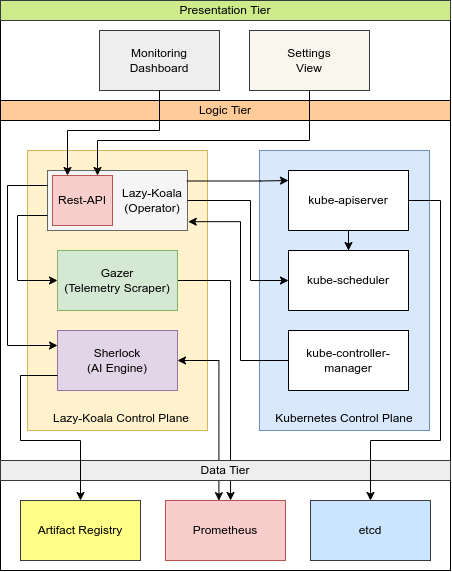
\includegraphics[width=14cm]{assets/system-design/tier-architecture.png}
    \caption{Tiered architecture (self-composed))}
    \label{fig:tier-architecture}
\end{figure}

\subsection{Presentation Tier}

The presentation tier will be entirely running in the client's computer while depending on the logic tier for data.

\begin{itemize}
    \item \textbf{Monitoring Dashboard} - This view is responsible for helping the user to understand the service topology and visually identify issues in the system.
    \item \textbf{Settings View} - On the settings page users can choose which services are needed to be monitored along with their DNS address.
\end{itemize}

\subsection{Logic Tier}

\begin{itemize}
    \item \textbf{Operator} - The operator is the main bridge between Kubernetes APIs and this system. It also contains a proxy server that securely redirects incoming client requests to kube-apiserver.
    \item \textbf{Gazer} - An instance of Gazer will be running on every node in the Kubernetes cluster which passively extracts telemetry and sends them over to the Prometheus server for later processing.
    \item \textbf{Sherlock} - AI engine periodically query Prometheus to get the current status of all the monitored service. Then it calculates an anomaly score for each service and pushes it to Prometheus so it can be sent back to the presentation layer
    \item \textbf{kube-apiserver} - This is an API provided by Kubernetes that help to read and update the cluster status programmatically.
    \item \textbf{kube-scheduler} - kube-scheduler is responsible for smartly provision requested resources in available spaces.
    \item \textbf{kube-controller-manager} - This service send updates to all the operators running on the cluster whenever there is a change to a resource that was owned by the specific operator.
\end{itemize}

\subsection{Data Tier}

\begin{itemize}
    \item \textbf{Artifact registry} - All the pre-trained models and built containers will be saved here for easy access.
    \item \textbf{Prometheus} - Prometheus is a time-series database that is highly optimized for storing service telemetry.
    \item \textbf{etcd} - etcd is an in-memory database that will be responsible for holding the resources specifications and Gazer config.
\end{itemize}